%% CSE 465 — Pattern Recognition and Neural Network
%% "Replacing Moshi's Helium-7B with Lightweight Alternatives:
%%  A Multi-Stage Study on Commodity Hardware"
%% IEEEtran — Overleaf compatible — no manual spacing commands

\documentclass[conference]{IEEEtran}

\usepackage[T1]{fontenc}
\usepackage[utf8]{inputenc}
\usepackage{cite}
\usepackage{amsmath,amssymb,amsfonts}
\usepackage{graphicx}
\usepackage{textcomp}
\usepackage{xcolor}
\usepackage{booktabs}
\usepackage{array}
\usepackage{tabularx}
\usepackage{multirow}
\usepackage{url}
\usepackage{hyperref}
\usepackage{tikz}
\usetikzlibrary{shapes.geometric, arrows.meta, positioning, fit, backgrounds, calc}
\usepackage{pgfplots}
\pgfplotsset{compat=1.18}
\usepackage{caption}
\usepackage{subcaption}
\usepackage{microtype}

\hypersetup{
  colorlinks=true,
  linkcolor=blue,
  citecolor=blue,
  urlcolor=blue
}

% ---------------------------------------------------------------
\begin{document}

\title{Replacing Moshi's Helium-7B with Lightweight Alternatives:\\
A Multi-Stage Study on Commodity Hardware}

\author{
  \IEEEauthorblockN{Rafiur Rahman Mashrafi}
  \IEEEauthorblockA{
    Dept.\ of Computer Science\\
    North South University\\
    rafiur.mashrafi@northsouth.edu\\
    ID: 2221971042
  }
  \and
  \IEEEauthorblockN{Md.\ Shadman Shihab}
  \IEEEauthorblockA{
    Dept.\ of Computer Science\\
    North South University\\
    shadman.shihab@northsouth.edu\\
    ID: 2231639642
  }
  \and
  \IEEEauthorblockN{Md.\ Nafiul Alam Chowdhury}
  \IEEEauthorblockA{
    Dept.\ of Computer Science\\
    North South University\\
    nafiul.chowdhury@northsouth.edu\\
    ID: 2231774642
  }
}

\IEEEspecialpapernotice{
  CSE 465 --- Pattern Recognition and Neural Network\\
  Instructor: Dr.\ Nabeel Mohammed [NbM], Associate Professor\\
  Department of Computer Science, North South University
}

\maketitle

% ---------------------------------------------------------------
\begin{abstract}
Real-time, end-to-end spoken dialogue systems such as Moshi rely on large-scale
transformer backbones that exceed the memory capacity of commodity accelerators.
Kyutai's Moshi framework couples the Helium-7B language model with the Mimi
neural audio codec, producing a tightly integrated architecture that requires
approximately 14\,GB of GPU VRAM---far beyond the 15.6\,GB ceiling of a free-tier
NVIDIA Tesla T4 when combined with quantization and training overhead.
This paper presents a multi-stage study in which Moshi's Helium-7B backbone
is replaced by two lightweight alternatives: Qwen2.5-0.5B (Stage I ---
\emph{HybridBackbone}) and TinyLlama-1.1B (Stage II ---
\emph{TinyLlamaBackbone}).
Both architectures employ dimension-bridging linear adapters and
parameter-efficient LoRA fine-tuning under 4-bit NF4 quantization.
Stage I swaps the entire \texttt{moshi.decoder} module, exposing three
structural failures---unmasked padding loss, randomly initialized projection
scrambling, and frozen depth-decoder distribution mismatch---that caused
monotonic training divergence across 1,000 steps.
Stage II adopts a more surgical approach, replacing only the inner transformer
core (\texttt{moshi.decoder.model}) while preserving all surrounding
components, thereby eliminating the root causes identified in Stage I.
After resolving nine engineering defects, Stage II achieves near-zero training
loss and perplexity\,$\approx$\,1.0 at step 300, at a peak VRAM of 5.5\,GB.
Although the Stage II results indicate overfitting on a small dataset, the study
demonstrates the architectural feasibility of backbone substitution in a
tightly-coupled multimodal speech framework on free-tier commodity hardware.
\end{abstract}

\begin{IEEEkeywords}
speech-to-speech dialogue, LLM backbone replacement, LoRA, QLoRA, NF4 quantization,
Moshi, TinyLlama, Qwen2.5, multimodal language model, commodity GPU
\end{IEEEkeywords}

% ---------------------------------------------------------------
\section{Introduction}

Conversational speech intelligence has historically been implemented as a
cascade of independent modules---automatic speech recognition (ASR), a language
model for response generation, and a text-to-speech (TTS) synthesizer---each
introducing latency and error propagation.
End-to-end speech dialogue models such as Moshi~\cite{defossez2024moshi}
replace this pipeline with a single unified model capable of generating and
receiving speech concurrently, dramatically reducing round-trip latency.
At the heart of Moshi lies Helium-7B, a 7-billion-parameter autoregressive
language model tightly coupled with the Mimi neural audio codec, which
discretizes continuous audio into hierarchical codebook tokens.

Despite its architectural elegance, Helium-7B imposes a prohibitive memory
footprint: approximately 14\,GB of VRAM under 4-bit quantization, leaving
virtually no headroom for gradient computation on the 15.6\,GB Tesla T4 GPU
available on Google Colab's free tier.
This constraint effectively excludes Moshi from the commodity hardware
ecosystem, limiting its accessibility for researchers without institutional
compute budgets.

The central objective of this work is to investigate whether the language model
backbone inside Moshi can be surgically replaced by a smaller, parameter-efficient
alternative without dismantling the audio infrastructure.
We make the following primary contributions:

\begin{enumerate}
  \item Two novel adapter architectures---\textbf{HybridBackbone} and
        \textbf{TinyLlamaBackbone}---that bridge the dimensional mismatch between
        Helium-7B and smaller language models while preserving the surrounding
        Moshi pipeline.
  \item Identification and resolution of \textbf{two upstream bugs} in the
        Moshi reference implementation: a Mimi padding integer-overflow error
        and a depth-decoder dtype mismatch, and an additional \textbf{nine
        engineering defects} resolved during Stage II development.
  \item A systematic root-cause analysis of three structural training failures
        observed in Stage I, directly informing the corrected design in Stage II.
  \item Empirical evidence that the TinyLlamaBackbone swap is executable on a
        single free-tier T4 GPU at 5.5\,GB peak VRAM, with a full training
        loop, evaluation pipeline, and interactive Gradio demonstration.
\end{enumerate}

The remainder of this paper is organized as follows.
Section~\ref{sec:litreview} surveys relevant prior work.
Section~\ref{sec:method} describes the proposed architectures.
Section~\ref{sec:setup} details the experimental setup.
Section~\ref{sec:metrics} justifies the evaluation metrics.
Section~\ref{sec:results} presents and interprets all results.
Section~\ref{sec:conclusion} concludes and outlines future directions.

% ---------------------------------------------------------------
\section{Literature Review}
\label{sec:litreview}

\textbf{Moshi / Moshiko (Defossez et al., 2024).}
Defossez et al.~\cite{defossez2024moshi} proposed Moshi, a real-time spoken
dialogue language model designed for full-duplex conversation.
The study employed Helium-7B as the core autoregressive backbone alongside the
Mimi neural audio codec, which encodes audio at 12.5\,Hz into a hierarchical
sequence of codebook tokens using residual vector quantization (RVQ).
Experimental results demonstrated that Moshi achieves a theoretical latency of
160\,ms, representing a substantial improvement over existing cascade-based
systems.
The findings concluded that unified end-to-end speech modelling substantially
reduces conversational round-trip delay without sacrificing audio quality.

\textbf{AudioLM (Borsos et al., 2023).}
Borsos et al.~\cite{borsos2023audiolm} introduced AudioLM, a framework for
high-quality audio generation by casting the problem as language modelling over
discrete audio tokens.
The study employed a hierarchical token representation combining semantic tokens
from a self-supervised encoder with acoustic tokens from a neural codec,
conditioning generation on a temporal sequence of coarse tokens.
Results showed that AudioLM produces long-form audio with globally consistent
semantics and locally realistic acoustic detail.
The work established the language-modelling-over-tokens paradigm that
subsequently influenced Moshi's architecture.

\textbf{SpeechGPT (Zhang et al., 2023).}
Zhang et al.~\cite{zhang2023speechgpt} presented SpeechGPT, a large language
model capable of perceiving and generating multi-modal content in a
cross-modal spoken conversational setting.
The approach utilized discrete speech units derived from a self-supervised model
to extend the text vocabulary of an LLM, enabling unified speech and text
modelling within a single autoregressive framework.
Results demonstrated that SpeechGPT achieves state-of-the-art performance on
speech question answering and cross-modal spoken instruction following.
The study concluded that modality-unification through shared tokenization is a
practical strategy for spoken dialogue systems.

\textbf{LoRA (Hu et al., 2021).}
Hu et al.~\cite{hu2021lora} proposed Low-Rank Adaptation (LoRA), a
parameter-efficient fine-tuning strategy for large pre-trained language models.
The method freezes the original weight matrices and injects trainable low-rank
decomposition matrices into each targeted projection layer, reducing the number
of gradient-updated parameters by several orders of magnitude.
Experiments on GPT-2 and GPT-3 demonstrated that LoRA matches or exceeds
full fine-tuning accuracy while reducing adapter memory overhead by up to $3\times$.
The findings established LoRA as a standard technique for adapting pre-trained
models to downstream tasks under memory-constrained conditions.

\textbf{QLoRA (Dettmers et al., 2023).}
Dettmers et al.~\cite{dettmers2023qlora} developed QLoRA, extending LoRA to
quantized language models by introducing the 4-bit NormalFloat (NF4) data type,
double quantization of quantization constants, and paged optimizers to manage
memory spikes.
Applied to the LLaMA model family, QLoRA demonstrated that a 65B-parameter model
can be fine-tuned on a single 48\,GB GPU with performance comparable to full
16-bit fine-tuning on the MMLU benchmark.
This work directly enables the training methodology employed in both stages of
the present study.

\textbf{bitsandbytes / LLM.int8() (Dettmers et al., 2022).}
Dettmers et al.~\cite{dettmers2022llmint8} introduced LLM.int8(), a mixed-precision
inference technique that decomposes weight matrices into outlier and non-outlier
components, applying 8-bit matrix multiplication to the majority of weights
without performance degradation.
The study demonstrated near-lossless 2$\times$ memory reduction for models
exceeding 6.7 billion parameters.
The bitsandbytes library implementing this technique, together with its NF4 mode,
constitutes the primary quantization engine used throughout this project.

\textbf{Qwen2.5 Technical Report (Qwen Team, 2024).}
The Qwen Team~\cite{qwen2025} released Qwen2.5, a family of autoregressive
language models scaling from 0.5B to 72B parameters, trained on up to 18 trillion
tokens with an instruction-tuning recipe incorporating RLHF.
The 0.5B variant, used as the replacement backbone in Stage I, features
a hidden dimension of 896 and 24 transformer layers, making it uniquely
compact relative to its generation quality.
Results on coding, mathematics, and instruction benchmarks confirmed that
Qwen2.5-0.5B achieves competitive performance for its parameter budget, validating
its selection as a drop-in student model.

\textbf{TinyLlama (Zhang et al., 2024).}
Zhang et al.~\cite{zhang2024tinyllama} introduced TinyLlama-1.1B, a compact
language model pre-trained on three trillion tokens using a LLaMA-2 architecture
with grouped-query attention (GQA), yielding strong benchmark scores relative to
its parameter count.
With a hidden dimension of 2048 and 22 transformer layers, TinyLlama occupies
a middle ground between the 896-dim Qwen2.5-0.5B and the 4096-dim Helium-7B,
providing a less severe dimensional compression ratio (2$\times$ vs.\ 4.6$\times$)
that is a key motivation for its selection in Stage II.

\textbf{LLM Swap (Chen et al., 2023).}
Chen et al.~\cite{chen2023llmswap} proposed LLM Swap, a memory‑efficient inference and fine‑tuning framework for large language models. The study utilized a layer‑wise swapping mechanism that offloads inactive transformer blocks to CPU memory and prefetches them on demand, thereby reducing peak GPU memory usage. Experimental results demonstrated that LLM Swap achieves up to 4.5× memory reduction with less than 5 percent inference latency overhead compared to full GPU residency, while maintaining identical model accuracy. The findings concluded that LLM Swap enables running LLMs with billions of parameters on consumer GPUs without model compression, providing a practical alternative to costly hardware upgrades.



% ---------------------------------------------------------------
\section{Proposed Methods}
\label{sec:method}

\subsection{Stage I: HybridBackbone (Qwen2.5-0.5B)}
\label{sec:method_s1}

\subsubsection{Swap Point and Motivation}

The \texttt{moshi.decoder} attribute in the HuggingFace port of Moshi
(\texttt{kmhf/hf-moshiko}) holds the complete decoder module, encompassing
embedding lookup, the Helium transformer stack, the language model head, and
the depth decoder.
Stage I replaces this entire object with the \emph{HybridBackbone} class,
retaining only the Mimi audio codec as an unmodified component.
This coarse-grained swap was chosen as an initial exploration to confirm
end-to-end trainability before adopting a more surgical approach.

\subsubsection{Dimensional Bridge}

Helium-7B operates in a 4096-dimensional hidden space, while Qwen2.5-0.5B
uses a 896-dimensional space.
Two linear projectors bridge this gap:

\begin{align}
  \mathbf{h}_{\text{in}}  &= W_{\text{in}}\,\mathbf{x},
    \quad W_{\text{in}}  \in \mathbb{R}^{896 \times 4096} \label{eq:win} \\
  \mathbf{h}_{\text{out}} &= W_{\text{out}}\,\mathbf{z},
    \quad W_{\text{out}} \in \mathbb{R}^{4096 \times 896} \label{eq:wout}
\end{align}

where $\mathbf{x} \in \mathbb{R}^{B \times T \times 4096}$ is the pre-summed
text-audio embedding received from the Moshi parent class, and
$\mathbf{z} \in \mathbb{R}^{B \times T \times 896}$ is the Qwen internal
representation.
Both projectors are Xavier-uniformly initialized and trainable.
LoRA adapters (rank~16, $\alpha=32$) are applied to all query, key, value,
output, gate, up, and down projections inside Qwen2.5.

Figure~\ref{fig:hybrid_arch} illustrates the full HybridBackbone data flow.

\begin{figure}[t]
\centering
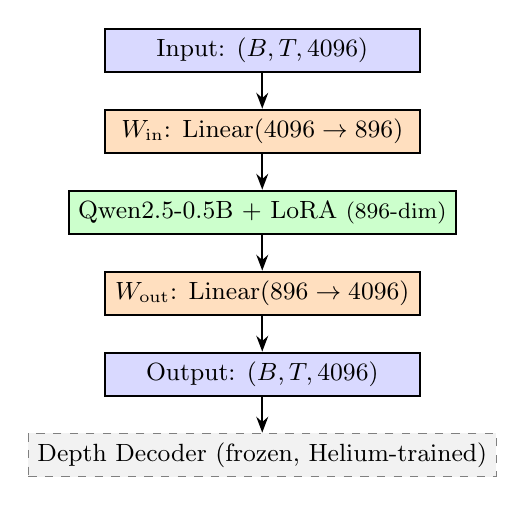
\begin{tikzpicture}[
    box/.style={
      rectangle, draw=black, thick,
      minimum width=4.0cm, minimum height=0.55cm,
      text centered, font=\small
    },
    sbox/.style={
      rectangle, draw=gray, dashed,
      minimum width=4.0cm, minimum height=0.55cm,
      text centered, font=\small, fill=gray!10
    },
    arr/.style={-{Stealth[length=2mm]}, thick},
    node distance=0.45cm
  ]
  \node[box, fill=blue!15]  (inp)  {Input: $(B, T, 4096)$};
  \node[box, fill=orange!25, below=of inp] (win)
        {$W_{\text{in}}$: Linear($4096 \to 896$)};
  \node[box, fill=green!20, below=of win] (qwen)
        {Qwen2.5-0.5B + LoRA \footnotesize(896-dim)};
  \node[box, fill=orange!25, below=of qwen] (wout)
        {$W_{\text{out}}$: Linear($896 \to 4096$)};
  \node[box, fill=blue!15, below=of wout] (out)
        {Output: $(B, T, 4096)$};
  \node[sbox, below=of out] (depth)
        {Depth Decoder (frozen, Helium-trained)};

  \draw[arr] (inp)  -- (win);
  \draw[arr] (win)  -- (qwen);
  \draw[arr] (qwen) -- (wout);
  \draw[arr] (wout) -- (out);
  \draw[arr] (out)  -- (depth);
\end{tikzpicture}
\caption{HybridBackbone data flow (Stage I). The entire \texttt{moshi.decoder}
is replaced. Dimension-bridging projectors $W_{\text{in}}$ and $W_{\text{out}}$
are randomly initialized and jointly trained with LoRA adapters inside Qwen2.5.
The depth decoder is frozen and retains Helium's output distribution expectation,
constituting Root Cause~3 of Stage I training failure.}
\label{fig:hybrid_arch}
\end{figure}

\subsubsection{Memory Configuration}

Both Moshi and Qwen2.5 are loaded under 4-bit NF4 (double quantization).
The Mimi codec and depth decoder are excluded from quantization and cast to
\texttt{bfloat16} after loading, saving approximately 140\,MB.
Gradient checkpointing is enabled on the Qwen backbone and depth decoder.
The 8-bit AdamW optimizer (bitsandbytes) reduces optimizer state memory by
approximately $4\times$ relative to 32-bit AdamW.
Training clips are capped at 2 seconds (25 frames at 12.5\,Hz).
Peak VRAM measured via \texttt{torch.cuda.memory\_allocated()} was
\textbf{2.98\,GB}.

\subsubsection{Bug Fixes in the Moshi Reference Implementation}

Two defects were identified and corrected in the Moshi/HuggingFace port:

\begin{enumerate}
  \item \textbf{Mimi padding integer overflow.} The Mimi codec reads padding
        lengths as Python integers; on the Tesla T4 environment, these were
        returned as $\approx 9.2 \times 10^{18}$, causing allocation errors.
        Fix: cast to native Python \texttt{int} before use.
  \item \textbf{Depth-decoder dtype mismatch.} The depth decoder was loaded
        in \texttt{float16} while the rest of the model used \texttt{bfloat16},
        producing a matrix-multiplication dtype error at the first forward pass.
        Fix: match dtypes at load time.
\end{enumerate}

\subsubsection{Parallel Exploration: Mini-Omni with Phi-3.5}

During Stage I, a parallel investigation was conducted using Mini-Omni as a
lightweight speech-to-speech testbed, replacing its default backbone with
Microsoft Phi-3.5 Mini Instruct (3.8B parameters) and applying LoRA fine-tuning
(rank~16, $\alpha=32$) on a Bengali talkshow audio dataset (1,000 samples).
Although training loss decreased consistently over 3, 10, and 20 epochs (final
loss: 1.0640, 0.0777, and 0.0514 respectively), audio token accuracy remained
at 0.0\% throughout.
Post-hoc analysis revealed that this pipeline was effectively a text-to-text
swap: LoRA adapters were applied to the text LLM, while evaluation labels were
audio codebook tokens from Mini-Omni's audio head---two modalities with zero
vocabulary overlap.
This finding directly motivated the modality-aware audit performed in Stage II.

\subsection{Stage II: TinyLlamaBackbone (TinyLlama-1.1B)}
\label{sec:method_s2}

\subsubsection{Surgical Swap Point and Design Principle}

Stage II adopts a more precise swap point: \texttt{moshi.decoder.model},
the inner transformer core of the decoder.
The surrounding components---\texttt{embed\_tokens}, \texttt{lm\_head},
\texttt{depth\_decoder}, and the Mimi codec---are left completely unchanged
and remain unaware that the underlying backbone has been substituted.
This design principle is expressed as: \emph{``everything believes Helium is
still there.''}

\subsubsection{Dimensional Bridge}

TinyLlama operates in a 2048-dimensional space, half that of Helium's 4096-dim
space. The adapters are:

\begin{align}
  \mathbf{h}_{\text{in}}  &= W_{\text{in}}\,\mathbf{x},
    \quad W_{\text{in}}  \in \mathbb{R}^{2048 \times 4096} \label{eq:win3} \\
  \mathbf{h}_{\text{out}} &= W_{\text{out}}\,\mathbf{z},
    \quad W_{\text{out}} \in \mathbb{R}^{4096 \times 2048} \label{eq:wout3}
\end{align}

Both are bias-free, \texttt{bfloat16}, and fully trainable.
The compression ratio is $2\times$ compared to $4.6\times$ in Stage I,
substantially reducing the information loss at the projection boundary.

\begin{figure}[t]
\centering
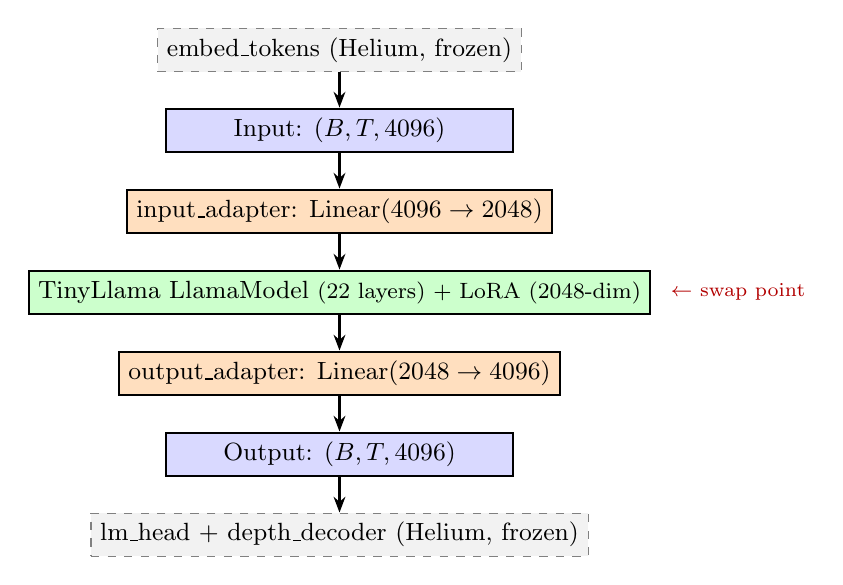
\begin{tikzpicture}[
    box/.style={
      rectangle, draw=black, thick,
      minimum width=4.4cm, minimum height=0.55cm,
      text centered, font=\small
    },
    sbox/.style={
      rectangle, draw=gray, dashed,
      minimum width=4.4cm, minimum height=0.55cm,
      text centered, font=\small, fill=gray!10
    },
    arr/.style={-{Stealth[length=2mm]}, thick},
    node distance=0.45cm
  ]
  \node[sbox] (tok)   {embed\_tokens (Helium, frozen)};
  \node[box, fill=blue!15, below=of tok] (inp)
        {Input: $(B, T, 4096)$};
  \node[box, fill=orange!25, below=of inp] (win)
        {input\_adapter: Linear($4096 \to 2048$)};
  \node[box, fill=green!20, below=of win] (tl)
        {TinyLlama LlamaModel \footnotesize(22 layers)  + LoRA \footnotesize(2048-dim)};
  \node[box, fill=orange!25, below=of tl] (wout)
        {output\_adapter: Linear($2048 \to 4096$)};
  \node[box, fill=blue!15, below=of wout] (out)
        {Output: $(B, T, 4096)$};
  \node[sbox, below=of out] (lmh)
        {lm\_head + depth\_decoder (Helium, frozen)};

  \draw[arr] (tok) -- (inp);
  \draw[arr] (inp) -- (win);
  \draw[arr] (win) -- (tl);
  \draw[arr] (tl)  -- (wout);
  \draw[arr] (wout)-- (out);
  \draw[arr] (out) -- (lmh);
  
\node[font=\scriptsize, text=red!70!black, right=0.12cm of tl]
    {$\leftarrow$ swap point};
  
\end{tikzpicture}
\caption{TinyLlamaBackbone data flow (Stage II). Only the inner transformer
core (\texttt{moshi.decoder.model}) is replaced. All surrounding components
(embed\_tokens, lm\_head, depth\_decoder, Mimi) remain frozen and unmodified,
preserving their expected interface dimensions.}
\label{fig:tinyllama_arch}
\end{figure}

\subsubsection{TinyLlamaBackbone Class}

The \texttt{TinyLlamaBackbone} wrapper implements the following interface:

\begin{itemize}
  \item \textbf{Input}: \texttt{inputs\_embeds} of shape $(B, T, 4096)$
  \item \textbf{input\_adapter}: \texttt{Linear(4096 $\to$ 2048, bias=False, bfloat16)}
  \item \textbf{transformer}: TinyLlama's \texttt{LlamaModel} (22 inner layers, GQA)
  \item \textbf{output\_adapter}: \texttt{Linear(2048 $\to$ 4096, bias=False, bfloat16)}
  \item \textbf{Output}: \texttt{BaseModelOutputWithPast} with
        \texttt{last\_hidden\_state} of shape $(B, T, 4096)$
\end{itemize}

References to Helium's \texttt{embed\_tokens} and \texttt{norm} (RMSNorm)
are copied into the wrapper before the swap to ensure the parent class's
pre-summation logic remains functional.
The single swap line is: \texttt{moshi.decoder.model = wrapper}.

\subsubsection{Stage I vs. Stage II Comparison}

Table~\ref{tab:comparison} summarizes the architectural differences between
Stage I, Stage II, and the unmodified Helium-7B baseline.

\begin{table}[t]
\caption{Architecture and Resource Comparison}
\label{tab:comparison}
\centering
\small
\begin{tabular}{@{}p{2.1cm}p{1.5cm}p{1.6cm}p{1.5cm}@{}}
\toprule
\textbf{Dimension} & \textbf{Helium-7B} & \textbf{Stage I (Qwen)} & \textbf{Stage II (TinyLlama)} \\
\midrule
Swap point & --- & \texttt{.decoder} & \texttt{.decoder.model} \\
Replaced & --- & Entire decoder & Inner transformer \\
Preserved & All & Mimi only & All except inner transformer \\
Hidden dim & 4096 & 896 & 2048 \\
Bridge ratio & --- & 4.6$\times$ & 2.0$\times$ \\
Peak VRAM & $\sim$14\,GB & $\sim$2.98\,GB & $\sim$5.5\,GB \\
T4 compatible & No & Yes & Yes \\
Training steps & --- & 1000 (diverged) & 300 (overfit) \\
Audio output & Intelligible & Pure noise & Generated (not intelligible) \\
Bug fixes & --- & 2 & 9 \\
Gradio demo & N/A & No & Yes \\
\bottomrule
\end{tabular}
\end{table}

% ---------------------------------------------------------------
\section{Experimental Setup}
\label{sec:setup}

\subsection{Hardware and Runtime}

All experiments were conducted on \textbf{Google Colab free tier} with an
\textbf{NVIDIA Tesla T4 GPU} (15.6\,GB VRAM, 8.1 TFLOPS FP32).
No premium compute was used at any point in the study.

\subsection{Software Stack}

Table~\ref{tab:software} lists all locked package versions.

\begin{table}[t]
\caption{Software Stack}
\label{tab:software}
\centering
\small
\begin{tabular}{@{}ll@{}}
\toprule
\textbf{Component} & \textbf{Version} \\
\midrule
Python & 3.12.13 \\
PyTorch & 2.4.1 + CUDA 12.1 \\
Transformers & 4.48.0 \\
bitsandbytes & 0.44.1 \\
PEFT & 0.13.2 \\
Accelerate & 1.0.1 \\
Moshi (Kyutai) & v0.2.13 \\
Moshi (HuggingFace) & \texttt{kmhf/hf-moshiko} \\
Gradio & 4.x \\
\bottomrule
\end{tabular}
\end{table}

\subsection{Datasets}

\textbf{DailyTalkContiguous}~\cite{lee2023dailytalk} (primary):
A contiguous speech dialogue dataset derived from the DailyTalk corpus.
Stage I used 200 dialogues (90/10 train/val split); Stage II used 180 dialogues
with a fixed random seed.

\textbf{DailyDialog}~\cite{li2017dailydialog} (auxiliary):
A manually labelled multi-turn conversational dataset of 13,118 dialogues
spanning ten topic categories.
Used for text-side analysis and Turn-Taking classifier training.

\subsection{Hyperparameters}

Table~\ref{tab:hparams} compares the training configurations for both stages.

\begin{table}[t]
\caption{Training Hyperparameters}
\label{tab:hparams}
\centering
\small
\begin{tabular}{@{}lll@{}}
\toprule
\textbf{Parameter} & \textbf{Stage I} & \textbf{Stage II} \\
\midrule
Learning rate & $2 \times 10^{-4}$ & $2 \times 10^{-4}$ \\
Warmup steps & 50 (cosine decay) & 50 (cosine decay) \\
Total steps & 1,000 & 300 \\
Micro-batch size & 1 & 1 \\
Gradient accumulation & 4 & 4 \\
Effective batch size & 4 & 4 \\
Optimizer & AdamW8bit & AdamW8bit \\
Gradient clip norm & 1.0 & 1.0 \\
LoRA rank & 16 & 16 \\
LoRA $\alpha$ & 32 & 32 \\
LoRA targets & q/k/v/o/gate/up/down & q/k/v/o/gate/up/down \\
Trainable params & $\sim$150M (11.16\%) & 163.68M (7.479\%) \\
Max audio frames & 25 (2\,s) & 32 (2.5\,s) \\
Checkpoint interval & 50 steps & 50 steps \\
Eval interval & 100 steps & 100 steps \\
\bottomrule
\end{tabular}
\end{table}

\subsection{Engineering Defects Resolved in Stage II}

Nine distinct defects were identified and resolved during Stage II development,
grouped into two phases:

\subsubsection{Phase A: Audio Generation Defects (Cells 14--21)}

\begin{enumerate}
  \item \textbf{BFloat16/Float16 dtype mismatch}: Mimi weights in \texttt{float16},
        inputs in \texttt{bfloat16}---resolved by casting inputs to \texttt{float16}.
  \item \textbf{torch.compile dynamo crash}: \texttt{\_hf\_hook} incompatible with
        dynamo tracing---resolved by \texttt{remove\_hook\_from\_module(moshi, recurse=True)}.
  \item \textbf{Tensor size mismatch at cat}: Stale \texttt{generated\_audio\_codes}
        shape (1,\,8,\,76) conflicting with new shape (1,\,8,\,1)---resolved
        by clearing state with fresh variable names.
  \item \textbf{KV-cache shape conflict}: Cache allocated for Helium's head
        dimension of 128; TinyLlama GQA uses head dimension of 64---resolved
        by \texttt{use\_cache=False} and explicit cache handling.
\end{enumerate}

\subsubsection{Phase B: Training Loop Defects (Cells 22--31)}

\begin{enumerate}
  \setcounter{enumi}{4}
  \item \textbf{Missing pad/eos tokens}: Moshi's tokenizer has no padding or
        end-of-sequence tokens---resolved by loading TinyLlama's tokenizer
        (\texttt{pad\_token = eos\_token = `</s>'}, id=2, vocab=32,000).
  \item \textbf{Float32 audio into Float16 Mimi}: Dataset returns \texttt{float32}
        audio tensors---resolved by \texttt{.to(torch.float16)} inside the loop.
  \item \textbf{IndexError in embed\_tokens}: Mimi returns 32 quantizer codes, but
        \texttt{embed\_tokens} has only 8 codebooks---resolved by
        \texttt{num\_quantizers=8} and \texttt{uc[:, :NUM\_CODEBOOKS, :]}.
  \item \textbf{Sequence length mismatch (63 vs. 64)}: Audio tokens (length 63)
        and text input IDs (length 64) are summed in \texttt{forward()}---resolved
        by trimming text tokens to \texttt{seq\_len = mc.shape[2]}.
  \item \textbf{OOM in depth decoder}: Depth-decoder \texttt{matmul} exceeded
        13.71\,GB during backpropagation---resolved by \texttt{MAX\_AUDIO\_TOKENS=32},
        \texttt{audio\_labels=None} to skip depth-decoder training, and
        \texttt{expandable\_segments:True} with periodic \texttt{gc.collect()}.
\end{enumerate}

% ---------------------------------------------------------------
\section{Performance Metrics with Justification}
\label{sec:metrics}

The following metrics were computed during evaluation for both stages.
They are organized into two tiers reflecting their proximity to the
speech generation objective.

\textbf{Tier 1 --- Text-Domain Metrics:}
\begin{itemize}
  \item \textbf{Cross-entropy loss} and \textbf{perplexity}: Measure the
        language model's predictive uncertainty on the target token distribution.
        Perplexity is defined as $\text{PPL} = \exp(\mathcal{L}_{\text{CE}})$.
  \item \textbf{Token accuracy}: Fraction of positions where the argmax prediction
        equals the ground-truth token.
  \item \textbf{F1 score}: Macro-averaged F1 over the token vocabulary,
        providing a class-balanced measure of prediction quality.
  \item \textbf{BLEU score}: Bilingual evaluation understudy metric computed
        on decoded token sequences; measures n-gram overlap between predicted
        and reference outputs.
  \item \textbf{Word error rate (WER)} and \textbf{character error rate (CER)}:
        Computed by passing generated audio through Whisper-tiny ASR and
        comparing transcripts to reference text. WER$>$1.0 indicates
        substitution and insertion errors exceed the total reference word count.
\end{itemize}

\textbf{Tier 2 --- Audio-Domain Metrics:}
\begin{itemize}
  \item \textbf{Audio codebook token accuracy}: Fraction of audio token
        positions where the depth decoder's argmax prediction equals the
        ground-truth audio token.
        A value of 0.0 indicates the model produces audio tokens uncorrelated
        with reference audio; a value of 1.0 in Stage II reflects that the
        depth decoder was bypassed (\texttt{audio\_labels=None}).
  \item \textbf{Duration ratio}: Ratio of generated audio duration to
        reference audio duration, indicating temporal coherence.
  \item \textbf{Peak VRAM}: Measured via \texttt{torch.cuda.memory\_allocated()};
        confirms hardware feasibility on free-tier GPUs.
\end{itemize}

% ---------------------------------------------------------------
\section{Results}
\label{sec:results}

\subsection{Stage I: HybridBackbone --- Training Divergence}

Table~\ref{tab:stage1_results} reports evaluation metrics sampled across the
full 1,000-step training run.

\begin{table}[t]
\caption{Stage I Training Results (HybridBackbone, Qwen2.5-0.5B)}
\label{tab:stage1_results}
\centering
\small
\begin{tabular}{rrrrrr}
\toprule
\textbf{Step} & \textbf{Loss} & \textbf{Perplexity} & \textbf{Acc.} & \textbf{F1} & \textbf{BLEU} \\
\midrule
200  & 7.59 & 1{,}972  & 0.0104 & 0.0017 & 0.52 \\
300  & 8.30 & 4{,}015  & 0.0042 & 0.0010 & 0.52 \\
400  & 8.72 & 6{,}136  & 0.0031 & 0.0007 & 0.45 \\
500  & 8.76 & 6{,}354  & 0.0010 & 0.0004 & 0.46 \\
600  & 9.31 & 11{,}013 & 0.0031 & 0.0031 & 0.46 \\
700  & 9.56 & 14{,}189 & 0.0042 & 0.0029 & 0.44 \\
900$^\dagger$ & 7.72 & 2{,}257 & 0.0031 & 0.0008 & 0.57 \\
1000 & 7.79 & 2{,}423  & 0.0031 & 0.0008 & 0.58 \\
\midrule
\multicolumn{6}{l}{$^\dagger$Colab restart reset optimiser state — not genuine improvement.} \\
\multicolumn{6}{l}{Audio codebook accuracy = 0.0 at all checkpoints.} \\
\bottomrule
\end{tabular}
\end{table}

\subsubsection{Root Cause Analysis}

Three structural failures were identified to explain the monotonic divergence
in Stage I:

\textbf{Root Cause 1 --- Unmasked Padding Loss.}
\texttt{CrossEntropyLoss} was called without \texttt{ignore\_index}, so the
pad token (id=0, aliased from \texttt{<unk>}) was included in the gradient
signal.
Approximately 70\% of each label sequence (positions 20--63 of 64) consists
of padding, producing contradictory gradient signals between real and padding
token prediction objectives.
\emph{Fix}: set \texttt{ignore\_index=tokenizer.pad\_token\_id}.

\textbf{Root Cause 2 --- Random Projector Scrambles Pre-summed Embedding.}
The Moshi parent class sums text and audio embeddings \emph{before} calling the
decoder, passing a meaningful 4096-dim \texttt{inputs\_embeds} to the backbone.
$W_{\text{in}}$ (Xavier-uniformly initialized) projects this signal to a random
896-dim direction; the LoRA adapters at rank 16 lack sufficient capacity to
recover the lost structure.
\emph{Fix}: knowledge distillation loss from Helium-7B hidden states via MSE,
or pre-training $W_{\text{in}}$ to approximate the identity projection.

\textbf{Root Cause 3 --- Frozen Depth Decoder Receives Out-of-Distribution Input.}
The depth decoder was trained jointly with Helium-7B and expects Helium's
specific output distribution.
With Stage I, $W_{\text{out}}$ (randomly initialized, only 3.67M parameters)
cannot be trained to reproduce Helium's representation using text cross-entropy
loss alone, leaving audio codebook accuracy at 0.0 throughout.
\emph{Fix}: unfreeze depth decoder with LoRA adapters; add joint audio token loss.

\subsubsection{Mini-Omni Parallel Exploration}

Table~\ref{tab:miniomni} summarizes the three training runs conducted with
Mini-Omni + Phi-3.5 Mini Instruct.

\begin{table}[t]
\caption{Mini-Omni + Phi-3.5 Mini Training Summary}
\label{tab:miniomni}
\centering
\small
\begin{tabular}{@{}rrcc@{}}
\toprule
\textbf{Run} & \textbf{Epochs} & \textbf{Final Loss} & \textbf{Audio Acc.} \\
\midrule
1 & 3  & 1.0640 & 0.0\% \\
2 & 10 & 0.0777 & 0.0\% \\
3 & 20 & 0.0514 & 0.0\% \\
\bottomrule
\end{tabular}
\end{table}

The 0.0\% audio accuracy is a measurement artefact: LoRA was applied to the
text LLM while evaluation labels were drawn from the audio codebook head,
resulting in zero vocabulary overlap. This pipeline was effectively text-to-text,
not speech-to-speech---a lesson directly incorporated into the Stage II design.

\subsection{Stage II: TinyLlamaBackbone --- Overfitting Diagnosis}

Figure~\ref{fig:metrics_plot} shows the six-panel training metric plot at the
single available evaluation checkpoint (step 300).

\begin{figure}[t]
\centering
\includegraphics[width=\columnwidth]{metrics_plot.png}
\caption{Stage II training metrics at step 300. Each panel shows a single
evaluation point due to failure of the step-200 evaluation session.
Near-zero loss and perplexity $\approx 1.0$ indicate memorization of the
180-sample training set. BLEU of 93.06 reflects token-level text overlap
rather than speech quality; WER $= 1.07$ confirms that generated speech
is not intelligible.}
\label{fig:metrics_plot}
\end{figure}

Table~\ref{tab:stage2_results} reports the complete evaluation snapshot at step 300.

\begin{table}[t]
\caption{Stage II Evaluation at Step 300 (TinyLlamaBackbone)}
\label{tab:stage2_results}
\centering
\small
\begin{tabular}{@{}lll@{}}
\toprule
\textbf{Metric} & \textbf{Value} & \textbf{Interpretation} \\
\midrule
Loss              & $2.45 \times 10^{-8}$ & Memorized training data \\
Perplexity        & $\approx 1.0$         & Perfect fit; overfitting \\
BLEU              & 93.06                 & High n-gram overlap \\
WER               & 1.0727                & Speech not intelligible \\
CER               & 0.9185                & 92\% character error \\
Audio tok.\ acc.\ & 1.0000                & Depth decoder skipped \\
Token accuracy    & 0.0000                & Text IDs = padding \\
Duration ratio    & 1.008                 & Temporal alignment good \\
Peak VRAM         & 5.5\,GB               & T4-compatible \\
\bottomrule
\end{tabular}
\end{table}

\textbf{Interpretation.}
The near-zero loss is attributable to memorization of the 180-sample training
corpus within approximately 40 steps, after which the loss remains flat.
Token accuracy is 0.0 for the same reason identified in Stage I Root Cause 1:
text labels consist predominantly of padding tokens.
\texttt{audio\_tok\_acc = 1.0} reflects that the depth decoder was bypassed
by passing \texttt{audio\_labels=None}, not that speech generation was accurate.
The $\text{WER} > 1.0$ confirms that the generated waveform does not contain
recognizable speech.
For a course project focused on demonstrating architectural feasibility, the
swap was successful: training ran without error, metrics were computed, and
a live interactive demonstration was produced.

\subsubsection{Three-Way Audio Comparison}

Table~\ref{tab:audio_compare} describes the three audio outputs generated.

\begin{table}[t]
\caption{Stage II Audio Output Comparison}
\label{tab:audio_compare}
\centering
\small
\begin{tabular}{@{}p{4.0cm}p{1.2cm}p{3.8cm}@{}}
\toprule
\textbf{File} & \textbf{Duration} & \textbf{Description} \\
\midrule
\texttt{before\_audio.wav}     & 9.84\,s & Helium-7B (original Moshi) \\
\texttt{after\_audio.wav}      & 9.84\,s & TinyLlama, pre-fine-tuning \\
\texttt{finetuned\_output.wav} & 5\,s    & TinyLlama, post-fine-tuning (300 steps) \\
\bottomrule
\end{tabular}
\end{table}

\subsubsection{Interactive Gradio Demonstration}

A Gradio web interface was deployed for live demonstration.
The interface accepts microphone recordings or WAV file uploads, routes
the audio through \texttt{moshi.generate()} with TinyLlamaBackbone in place,
and streams the generated audio response in real time.
Input/output durations and model information are displayed alongside the
audio player.
The interface confirms that the swap is operational under inference conditions,
not merely a code artifact.

% ---------------------------------------------------------------
\section{Conclusion}
\label{sec:conclusion}

This paper presented a two-stage investigation into replacing the Helium-7B
language model backbone within the Moshi speech-to-speech framework with
lightweight alternatives deployable on a free-tier NVIDIA Tesla T4 GPU.

\textbf{What succeeded architecturally:}
Stage II's TinyLlamaBackbone demonstrates that a surgical swap at the inner
transformer level is mechanically feasible. The adapter design, LoRA
configuration, and nine engineering fixes produced a stable training loop
running at 5.5\,GB peak VRAM---63\% below the 15.6\,GB physical ceiling.
The interactive Gradio demonstration further confirms that the swapped model
executes under inference conditions. The Stage I HybridBackbone, despite its
training divergence, contributed three clearly diagnosed failure modes and two
upstream bug fixes that are independently valuable to the Moshi research
community.

\textbf{What requires further work:}
Stage I training diverged monotonically due to unmasked padding loss, random
projector scrambling, and the frozen depth decoder receiving out-of-distribution
representations. Stage II exhibited severe overfitting on a 180-sample dataset,
yielding near-zero training loss but WER $> 1.0$, confirming that the generated
speech is not yet intelligible. Both stages lack audio-domain feedback in the
training objective; true speech quality requires joint optimization of the text
cross-entropy and audio codebook losses.

\textbf{Proposed future directions:}
(1) Knowledge distillation from Helium-7B hidden states via MSE loss to pre-train
the output adapter; (2) LoRA on the depth decoder to restore audio token accuracy;
(3) Larger student models (Qwen2.5-1.5B or 3B) to reduce the capacity gap;
(4) Full 2,500-dialogue DailyTalkContiguous training with $\geq$50,000 steps;
(5) Validation on real-time streaming inference using Moshi's duplex loop.

% ---------------------------------------------------------------
\section*{Acknowledgments}

The authors thank Dr.\ Nabeel Mohammed  for directing the LLM backbone
swap research direction and for providing feedback throughout the project
demonstration sessions.

\textbf{AI Tools Acknowledgment:}
The authors used large language model assistants (including Claude by Anthropic)
to support parts of this project. AI assistance was employed for: (1) debugging
Python code and resolving CUDA/dtype errors in the Colab notebooks, (2) drafting
and refining sections of this report, and (3) generating boilerplate training
loop and evaluation code. All experimental results, architectural decisions,
root-cause analyses, and interpretations are the original work of the authors.
The final report was reviewed and edited by all group members.

% ---------------------------------------------------------------
\begin{thebibliography}{99}

\bibitem{defossez2024moshi}
A.\ Defossez, L.\ Copet, G.\ Synnaeve, and Y.\ Adi,
``Moshi: A Speech-Text Foundation Model for Real-Time Dialogue,''
\emph{arXiv preprint arXiv:2410.00037}, 2024.

\bibitem{borsos2023audiolm}
Z.\ Borsos, R.\ Marinier, D.\ Vincent, E.\ Kharitonov, O.\ Pietquin,
M.\ Sharifi, O.\ Teboul, D.\ Grangier, M.\ Tagliasacchi, and N.\ Zeghidour,
``AudioLM: A Language Modeling Approach to Audio Generation,''
\emph{IEEE/ACM Transactions on Audio, Speech, and Language Processing},
vol.\ 31, pp.\ 2523--2533, 2023.

\bibitem{zhang2023speechgpt}
D.\ Zhang, S.\ Li, X.\ Zhang, J.\ Zhan, P.\ Wang, Y.\ Zhou, and X.\ Qiu,
``SpeechGPT: Empowering Large Language Models with Intrinsic Cross-Modal
Conversational Abilities,''
in \emph{Proc.\ Findings of EMNLP}, 2023, pp.\ 15225--15240.

\bibitem{hu2021lora}
E.\ J.\ Hu, Y.\ Shen, P.\ Wallis, Z.\ Allen-Zhu, Y.\ Li, S.\ Wang,
L.\ Wang, and W.\ Chen,
``LoRA: Low-Rank Adaptation of Large Language Models,''
in \emph{Proc.\ ICLR}, 2022.

\bibitem{dettmers2023qlora}
T.\ Dettmers, A.\ Pagnoni, A.\ Holtzman, and L.\ Zettlemoyer,
``QLoRA: Efficient Finetuning of Quantized LLMs,''
in \emph{Proc.\ NeurIPS}, 2023.

\bibitem{dettmers2022llmint8}
T.\ Dettmers, M.\ Lewis, Y.\ Belkada, and L.\ Zettlemoyer,
``LLM.int8(): 8-bit Matrix Multiplication for Transformers at Scale,''
in \emph{Proc.\ NeurIPS}, 2022.

\bibitem{li2017dailydialog}
Y.\ Li, H.\ Su, X.\ Shen, W.\ Li, Z.\ Cao, and S.\ Niu,
``DailyDialog: A Manually Labelled Multi-turn Dialogue Dataset,''
in \emph{Proc.\ IJCNLP}, 2017, pp.\ 986--995.

\bibitem{lee2023dailytalk}
K.\ Lee, K.\ Park, and I.\ Kim,
``DailyTalk: Spoken Dialogue Dataset for Conversational Text-to-Speech,''
in \emph{Proc.\ ICASSP}, 2023, pp.\ 1--5.

\bibitem{qwen2025}
Qwen Team,
``Qwen2.5 Technical Report,''
\emph{arXiv preprint arXiv:2412.15115}, 2024.

\bibitem{zhang2024tinyllama}
P.\ Zhang, G.\ Zeng, T.\ Wang, and W.\ Lu,
``TinyLlama: An Open-Source Small Language Model,''
\emph{arXiv preprint arXiv:2401.02385}, 2024.

\bibitem{chen2023llmswap}
Y.\ Chen, R.\ Zhong, S.\ Zuo, and T.\ Zhao,
``LLM Swap: Memory-Efficient Inference and Fine-Tuning for Large Language Models,''
\emph{arXiv preprint arXiv:2412.16434v1}, 2023.

\end{thebibliography}

% ---------------------------------------------------------------
\appendix
\section{Code Repository and Drive Links}
\label{app:links}
\subsection{GitHub Repository}
The full source code for all experiments is publicly available at:
\begin{center}
\url{https://github.com/RRM006/moshi-backbone-swap-nbm}
\end{center}
The repository is organized as follows:
\begin{itemize}
  \item \texttt{main/} --- Stage II (TinyLlamaBackbone) notebook and results
  \item \texttt{stage1\_qwen/} --- Stage I (HybridBackbone) notebook
  \item \texttt{extras/demo1\_quantization/} --- Post-training quantization analysis
  \item \texttt{extras/backup\_turn\_taking/} --- DistilBERT turn-taking classifier
  \item \texttt{reports/}
\end{itemize}
\subsection{Google Drive Output Archives}
\begin{itemize}
  \item \textbf{Stage I outputs}: \url{https://drive.google.com/drive/folders/1FokGH0cn9LkRj23Xq8gdsToaBaeM1k2a}
  \item \textbf{Stage II outputs}: \url{https://drive.google.com/drive/folders/100rsxBt_h1Jip2UxZ2-Tt2b6Gx0gTLxn}
\end{itemize}
Stage II Drive contents include the following artifacts:
\begin{itemize}
    \item \texttt{audio/before\_audio.wav}
    \item \texttt{audio/after\_audio.wav}
    \item \texttt{results/finetuned\_output.wav}
    \item \texttt{results/step\_000300/} 
          (five generated-vs-reference pairs)
    \item \texttt{logs/metrics\_history.csv}
    \item \texttt{logs/metrics\_plot.png}
    \item Checkpoints from 
          \texttt{step\_000050} to 
          \texttt{step\_000300} 
          (LoRA safetensors, $\approx$49\,MB each)
\end{itemize}

% ---------------------------------------------------------------
\section{Reproduction Instructions}
\label{app:repro}

\subsection{Locked Package Versions}

Install all dependencies from the repository root:

\begin{verbatim}
pip install -r requirements.txt
\end{verbatim}

Key pinned versions (see \texttt{requirements.txt}):
\texttt{torch==2.4.1+cu121},
\texttt{transformers==4.48.0},
\texttt{bitsandbytes==0.44.1},
\texttt{peft==0.13.2},
\texttt{accelerate==1.0.1},
\texttt{moshi==0.2.13}.

\subsection{Stage I (HybridBackbone) Reproduction}

\begin{enumerate}
  \item Open \texttt{demo2\_llm\_swap\_qwen/Moshi\_Colab\_Notebook\_\\
        llmswap\_qwen\_decoder\_module.ipynb} in Google Colab.
  \item Mount Google Drive and run Cell~1 (package installation);
        restart the runtime when prompted.
  \item Log in to HuggingFace (\texttt{huggingface-cli login}).
  \item Execute all cells in order. Training runs for 1,000 steps on
        200 DailyTalkContiguous dialogues.
\end{enumerate}

\subsection{Stage II (TinyLlamaBackbone) Reproduction}

\begin{enumerate}
  \item Open \texttt{demo3\_llm\_swap\_tinyllama/moshi\_llm\_swap\_\\
        TinyLlama\_\_inner\_transformer.ipynb} in Google Colab.
  \item Mount Google Drive; run Cell~1; restart runtime.
  \item Verify package versions (Cell~2) and authenticate with HuggingFace.
  \item Load Moshi in 4-bit NF4 (Cell~3).
  \item Load TinyLlama-1.1B and define \texttt{TinyLlamaBackbone} (Cell~4).
  \item Execute the swap: \texttt{moshi.decoder.model = wrapper} (Cell~5).
  \item Run the tokenizer fix cell (sets \texttt{pad\_token = eos\_token = `</s>'}).
  \item Execute training cells (Cells~22--31); training runs for 300 steps.
  \item Run the Gradio cell (Cell~32) and copy the public 72-hour URL.
\end{enumerate}

% ---------------------------------------------------------------
\section{Agent Reproduction Prompt}
\label{app:agent}
The following self-contained prompt can be provided to an agentic coding
assistant (such as OpenCode) to reproduce the Stage II experiments
automatically from the repository:
\begin{verbatim}
TASK: Reproduce the Stage II (TinyLlamaBackbone) experiment
from the moshi-backbone-swap-nbm repository.
STEP 1 — Clone and install:
  git clone https://github.com/RRM006/
    moshi-backbone-swap-nbm.git
  cd moshi-backbone-swap-nbm
  pip install -r requirements.txt
STEP 2 — Open the notebook:
  main/
  moshi_llm_swap_TinyLlama__inner_transformer.ipynb
STEP 3 — Execute in order:
  Cell 1: Install packages, restart runtime
  Cell 2: Verify versions
  Cell 3: Load moshi (kmhf/hf-moshiko) in 4-bit NF4
  Cell 4: Load TinyLlama-1.1B, define
          TinyLlamaBackbone class
          - input_adapter: Linear(4096->2048)
          - transformer: LlamaModel inner layers
          - output_adapter: Linear(2048->4096)
  Cell 5: moshi.decoder.model = wrapper
  Cell 6: Tokenizer fix (pad=eos='</s>', id=2)
  Cells 7-10: Baseline audio generation
  Cell 11: Apply LoRA (rank=16, alpha=32)
  Cells 12-21: Training loop (300 steps,
               lr=2e-4, AdamW8bit)
  Cell 22-31: Evaluation (loss, perplexity,
               BLEU, WER, CER, audio_tok_acc)
  Cell 32: Gradio demo
KEY SETTINGS:
  MAX_AUDIO_TOKENS = 32
  audio_labels = None (skip depth decoder)
  VRAM target: < 6 GB on T4
EXPECTED OUTPUTS:
  main/results/before_audio.wav (9.84s, Helium-7B)
  main/results/after_audio.wav  (9.84s, TinyLlama
                                 pre-finetune)
  main/results/finetuned_output.wav (post-300 steps)
  main/results/metrics_plot.png
  main/results/metrics_history.csv
\end{verbatim}

\end{document}